\documentclass[aspectratio=169]{beamer}

\usepackage{../algpseudocodex}
\usepackage{amssymb}
\usepackage{biblatex}
\usepackage{listings}
\usepackage{mathtools}
\usepackage{subcaption}
\usepackage{tikz}

\addbibresource{../refs.bib}

\usetikzlibrary{graphs,graphdrawing}
\usegdlibrary{circular,trees}

\usetheme{metropolis}

\metroset{numbering=fraction,block=fill}
\setbeamertemplate{section in toc}[sections numbered]

\author{Leonard Techel}
\title{Low-Connectivity State Space Exploration using Swarm Model Checking on the GPU}
\date{August 12, 2021}

\begin{document}

\maketitle

\begin{frame}{Table of Contents}
    \tableofcontents
\end{frame}

\section{Motivation}

\begin{frame}{Motivation 1/4: Dining Philosophers}
    \vspace{.5cm}
    \begin{figure}
        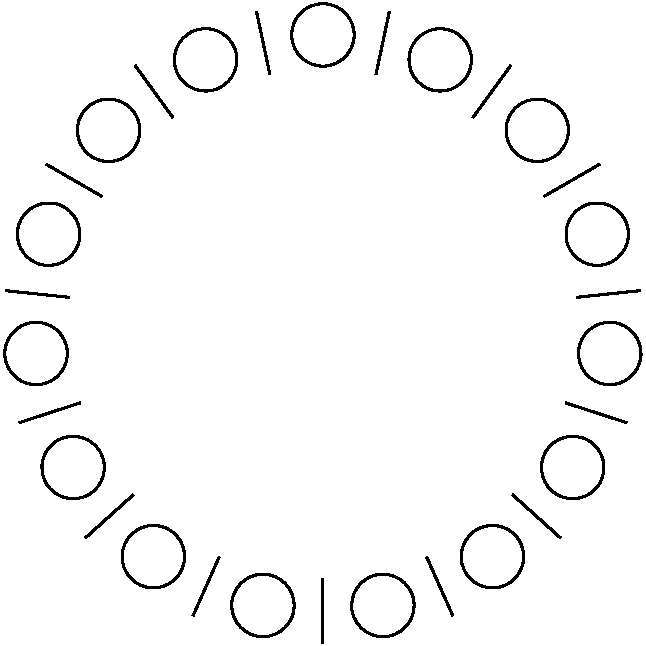
\includegraphics[width=.35\textwidth]{../figures/dining-philosophers}
        \caption{Dining Philosophers, $N=15$}
        \label{fig:dining-philosophers}
    \end{figure}
\end{frame}

\begin{frame}{Motivation 2/4: Dining Philosophers}
    \begin{columns}
        \begin{column}{.5\textwidth}
            \begin{itemize}
                \item 4 States
                \item Can only start eating when both forks are picked up
                \item \textbf{Goal:} Verify that there is never the case where all philosophers have picked up only the left fork, all waiting for each other
                \item How to do that algorithmically?
            \end{itemize}
        \end{column}
        \begin{column}{.5\textwidth}
            \begin{figure}
                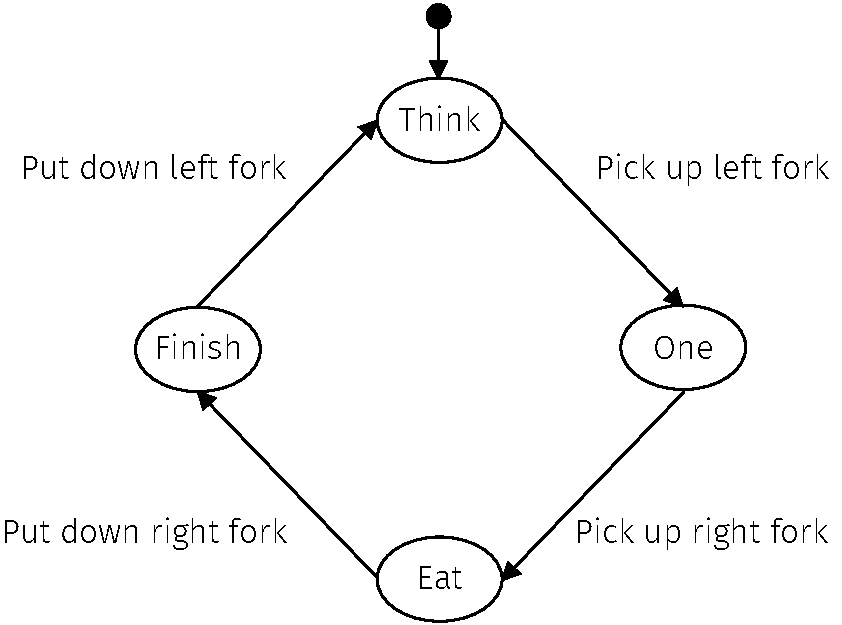
\includegraphics[width=\textwidth]{../figures/beamer-dining-philosopher-fsm}
                \caption{A dining philosopher's state machine}
                \label{fig:dining-philosopher-fsm}
            \end{figure}
        \end{column}
    \end{columns}
\end{frame}

\begin{frame}{Motivation 3/4: Verification}
    \begin{figure}
        \centering
        \begin{minipage}{.7\linewidth}
            \begin{algorithmic}
                \While{there are unvisited states}
                \State mark state as visited
                \If{state violates spec}
                \State report path to state
                \EndIf
                \EndWhile
            \end{algorithmic}
        \end{minipage}
        \vspace{\baselineskip}
        \caption{State Space Exploration Loop}
        \label{fig:state-space-exploration-loop}
    \end{figure}
\end{frame}

\begin{frame}{Motivation 4/4: Observations}
    \begin{itemize}
        \item We've invented a \emph{model checker}
        \item We have $3^{15}-1=14.348.906$ states to check
        \item Each state of the system needs at least $15\cdot2+15=45$ bit
        \item \textbf{Problem 1:} State Space Explosion
        \item \textbf{Problem 2:} State Space Exploration Loop gets slow quickly
        \item What can we do?
    \end{itemize}
\end{frame}

% \begin{frame}{Motivation 5/5}
%     Low-Connectivity State Space Exploration using Swarm Model Checking on the GPU

%     \begin{itemize}
%         \item State Space Exploration: \checkmark
%         \item Low-Connectivity: ?
%         \item Swarm Model Checking: ?
%         \item On the GPU: ?
%     \end{itemize}
% \end{frame}

\section{Model Checking, Swarm Verification}

\begin{frame}{Model Checking 1/3}
    \begin{itemize}
        \item Formal verification method
        \item The model checker finds out whether a state machine \emph{models} a specification
        \item Two branches: Explicit-State Model Checking and Symbolic Model Checking
        \item How does it work?
    \end{itemize}
\end{frame}

\begin{frame}{Model Checking 2/3: State Space Exploration Loop}
    \begin{columns}
        \begin{column}{.5\textwidth}
            \begin{figure}
                \centering\begin{algorithmic}
                    \While{there are unvisited states}
                    \State mark state as visited
                    \If{state violates spec}
                    \State report path to state
                    \EndIf
                    \EndWhile
                \end{algorithmic}
                % \caption{State Space Exploration Loop}
            \end{figure}
        \end{column}
        \begin{column}{.5\textwidth}
            \begin{itemize}
                \item Violating states are reported
                \item Typical algorithms: BFS / DFS
                \item Typical implementation: Single-Threaded
                \item How to make it faster?
            \end{itemize}
        \end{column}
    \end{columns}
\end{frame}

\begin{frame}{Model Checking 3/3: Parallelized Exploration Loop}
    \begin{itemize}
        \item Breadth-First Search can be parallelized
        \item \textbf{Problem:} Approaches use shared memory
        \item Scaling beyond a few thread: Communication overhead
        \item How can we scale onto massively parallel architectures, e.g. GPUs?
    \end{itemize}
\end{frame}

\begin{frame}{Swarm Verification 1/2}
    From the paper \emph{Swarm Verification} by G. J. Holzmann et al. \cite{Holzmann2008.Swarm-Verification}
    \begin{itemize}
        \item New approach on parallelized model checking
        \item \textbf{Idea:} Split state space exploration into small, independent tasks
        \item Tasks are called Verification Tests (VTs)
        \item Each VT only covers a subset of the state space
        \item \textbf{Result:} VTs can be massively parallelized on heterogeneous architectures
        \item How is the state space exploration split up?
    \end{itemize}
\end{frame}

\begin{frame}{Swarm Verification 2/2: Diversification Techniques}
    \begin{columns}
        \begin{column}{.5\textwidth}
            Diversification techniques:

            \begin{itemize}
                \item \textbf{Statistically independent hash functions}
                \item Reversing search order
                \item Randomizing order of nondeterministic choice
                \item \dots
            \end{itemize}

            Does it perform good?

            % How to run it on a GPU?
        \end{column}
        \begin{column}{.5\textwidth}
            \begin{figure}
                \begin{subfigure}[b]{.45\textwidth}
                    \resizebox{\textwidth}{!}{
                        \begin{tikzpicture}[nodes={draw, circle}]
                            \graph [tree layout, missing nodes get space] {
                                A [fill=lightgray];
                                B [fill=lightgray];
                                D [fill=lightgray];
                                E [fill=lightgray];
                                F [fill=lightgray];
                                I [fill=lightgray];
                                J [fill=lightgray];

                                A -- B [second];
                                A -- C;
                                A -- D;

                                B -- E;
                                B -- F;

                                C -- F;
                                C -- G;
                                C -- H;

                                D -- I;

                                F -- J;

                                H -- K;
                                H -- L;
                            };
                        \end{tikzpicture}
                    }
                    \subcaption*{Collision: \{B, C\}}
                \end{subfigure}
                \begin{subfigure}[b]{.45\textwidth}
                    \resizebox{\textwidth}{!}{
                        \begin{tikzpicture}[nodes={draw, circle}]
                            \graph [tree layout, missing nodes get space] {
                                A [fill=lightgray];
                                B [fill=lightgray];
                                C [fill=lightgray];
                                D [fill=lightgray];
                                E [fill=lightgray];
                                G [fill=lightgray];
                                H [fill=lightgray];
                                I [fill=lightgray];
                                K [fill=lightgray];
                                L [fill=lightgray];

                                A -- B;
                                A -- C;
                                A -- D;

                                B -- E;
                                B -- F;

                                C -- F;
                                C -- G;
                                C -- H;

                                D -- I;

                                F -- J;

                                H -- K;
                                H -- L;
                            };
                        \end{tikzpicture}
                    }
                    \subcaption*{Collision: \{E, F\}}
                \end{subfigure}
                \caption{State pruning using hash collisions}
                \label{figure:hash-collision-state-pruning}
            \end{figure}

        \end{column}
    \end{columns}
\end{frame}

\section{Low-Connectivity Models}

\begin{frame}{Low-Connectivity Models 1/3}
    \begin{itemize}
        \item Performance measure: \# of VTs to achieve nearly 100\% state space coverage
        \item When does it perform good?
              \begin{itemize}
                  \item Waypoints model
                        \begin{itemize}
                            \item 8 processes, each in control of 4 bits of a 32 bit int
                            \item On each transition, a process toggles one random bit
                            \item $2^{32} = \text{over 4 billion}$ states
                            \item 100 randomly distributed violations (waypoints)
                        \end{itemize}
                  \item Models with $<100\%$ hash table utilization
              \end{itemize}
        \item When does it perform less?
              \begin{itemize}
                  \item Low-Connectivity models
              \end{itemize}
    \end{itemize}
\end{frame}

\begin{frame}{Low-Connectivity Models 2/3: Definition}
    \begin{columns}
        \begin{column}{.6\textwidth}
            A model has \emph{low connectivity} if at least one of the following properties is satisfied:
            \begin{itemize}
                \item \textbf{Generally Linear}: The average \# of edges per state is close to 2: One inbound, one outbound
                \item \textbf{Bottleneck Structures}: A single state or group of states other than the initial state that needs to be passed to reach most of the state space
            \end{itemize}
        \end{column}
        \begin{column}{.4\textwidth}
            \begin{figure}
                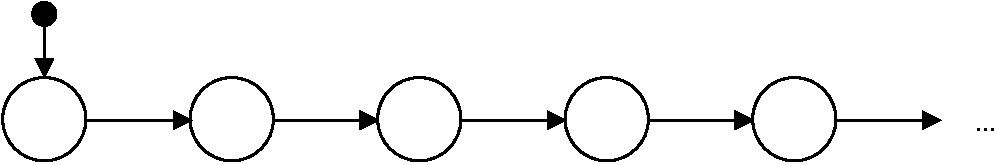
\includegraphics[width=.8\textwidth]{../figures/lc-ex-generally-linear}
                \caption{Example of a generally linear graph}
            \end{figure}
            \begin{figure}
                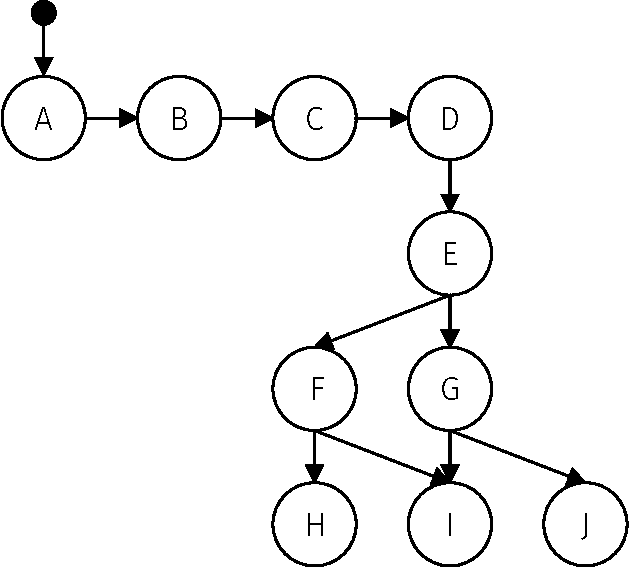
\includegraphics[width=.6\textwidth]{../figures/lc-ex-bottleneck}
                \caption{Example of a bottleneck structure}
            \end{figure}
        \end{column}
    \end{columns}
\end{frame}

\begin{frame}{Low-Connectivity Models 3/3: What to do?}
    \textbf{Goal:} Maximize the state space coverage while minimizing the amount of VTs to do so.
    \begin{enumerate}
        \item How can we (automatically) classify a model as low-connectivity?
        \item How can we improve the state space exploration of such models?
    \end{enumerate}

    How can Swarm Verification be implemented?
\end{frame}

\section{Implementation: CUDA, Grapple Model Checker}

\begin{frame}{Grapple Model Checker}
    From the paper \emph{Swarm model checking on the GPU} by R. DeFrancisco et al. \cite{DeFrancisco2020.Grapple}

    \begin{itemize}
        \item A framework for parallel Swarm Verification model checking on the GPU using CUDA
        \item Why GPUs? — GPUs are massively parallel, widely available and cheap
        \item What is CUDA?
    \end{itemize}
\end{frame}

\begin{frame}{CUDA 1/3}
    \begin{itemize}
        \item CUDA: NVIDIA's proprietary GPU programming framework
        \item Code is written in C/C++
        \item Automatic massive scalability
        \item How does the programming model work?
    \end{itemize}
\end{frame}

\begin{frame}{CUDA 2/3: Programming model}
    \begin{itemize}
        \item Write a \emph{kernel}
        \item Kernel execution: Define the amount of \emph{threads} and \emph{blocks}
        \item Each thread in a block executes the kernel in SIMT
        \item Each thread should work on a separate piece of memory
        \item GPU maps the blocks onto its \emph{streaming multiprocessors}
        \item Code example?
    \end{itemize}
\end{frame}

\begin{frame}[fragile]{CUDA 3/3: Code example}
    \begin{figure}
        \centering
        \begin{minipage}{.7\linewidth}
            \begin{lstlisting}[basicstyle=\scriptsize,language=c]
__global__ void VecAdd(float *A, float *B, float *C)
{
    int i = threadIdx.x;
    C[i] = A[i] + B[i];
}

int main(){
    ...
    VecAdd<<<1, N>>>(A, B, C);
}
            \end{lstlisting}
        \end{minipage}
        \caption{Add two arrays A, B of length $N$ in CUDA}
        \label{fig:cuda-add-arrays}
    \end{figure}

    How to do Swarm Verification on this architecture?
\end{frame}

\begin{frame}{Grapple Model Checker: Mapping to the CUDA architecture}

    \begin{itemize}
        \item Each VT's state space exploration runs in a parallel BFS
        \item Verification Tests: CUDA Blocks
        \item Worker in a VT: CUDA Thread
        \item Can it actually be implemented?
    \end{itemize}
\end{frame}

\begin{frame}{My implementation 1/2}
    \begin{itemize}
        \item \emph{It seems to work!}
        \item Currently only implements the \emph{Waypoints} benchmark model
        \item Hash table diversification seems not to be too good
        \item Philosophers model is on its way
    \end{itemize}
\end{frame}

\begin{frame}{My implementation 2/2: First results}
    $50.000$ runs, each with 250 VTs. Memory leak killed it after $\sim 16.000$ runs

    \begin{columns}
        \begin{column}{.5\textwidth}
            \begin{figure}
                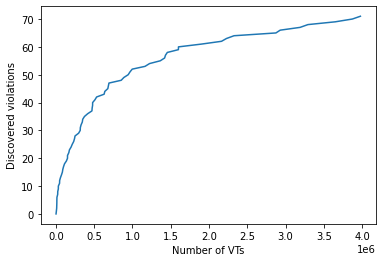
\includegraphics[width=\textwidth]{../figures/discovered-states-executed-vts}
                \caption{Number of discovered violations in relation to number of executed VTs}
                \label{fig:discovered-states-executed-vts}
            \end{figure}
        \end{column}
        \begin{column}{.5\textwidth}
            \begin{figure}
                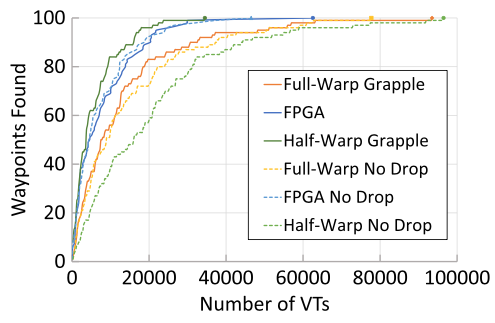
\includegraphics[width=\textwidth]{../figures/paper-discovered-states-executed-vts}
                \caption{Discovered waypoints in relation to executed VTs in the paper}
                \label{fig:paper-discovered-states-executed-vts}
            \end{figure}
            % \begin{figure}
            %     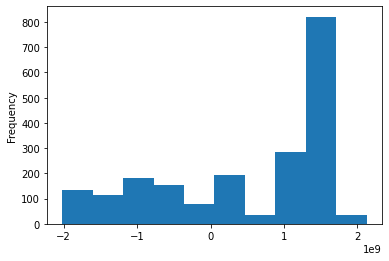
\includegraphics[width=\textwidth]{../figures/violating-states-frequency}
            %     \caption{Frequency of violating states}
            %     \label{fig:violating-states-frequency}
            % \end{figure}
        \end{column}
    \end{columns}
\end{frame}

\section{What's next?}

\begin{frame}{What's next?}
    \begin{itemize}
        \item Find out how the hash table collisions can be controlled better
        \item Study low-connectivity models more in-depth: Try out the different approaches from the paper (PDS, process-PDS, scatter-PDS, alternating between search strategies, …?)
    \end{itemize}
\end{frame}

\appendix

\begin{frame}{References} % [allowframebreaks]
    \printbibliography[heading=none]
\end{frame}

\end{document}
